\documentclass[letter,scriptaddress,twocolumn, prl,showkeys]{revtex4-1}

    \usepackage{microtype}
    \usepackage{blindtext}
    \usepackage{enumitem}
    \usepackage{siunitx}

	\usepackage{amsmath}%,amssymb} 
	\usepackage{makeidx}
	\usepackage{amsfonts}
	\usepackage[ansinew]{inputenc}
	\usepackage[usenames,dvipsnames]{pstricks}
	\usepackage{subfigure}
	\usepackage{epsfig}
%	\usepackage{pst-grad} % For gradients
	\usepackage{pst-plot} % For axes
	\usepackage[colorlinks,hyperindex]{hyperref}
    \usepackage{color}
	\hypersetup
	{
		colorlinks,%
		citecolor=black,%
		linkcolor=black,%
		urlcolor=black,%
	}

%--- Theorem like environments ----
	\newtheorem{theorem}{Theorem}
	\newtheorem{corolary}{Corolary}
	\newtheorem{prop}{Proposition}
	\newtheorem{definition}{Definition}
	\newtheorem{example}{Example}
	\newtheorem{exercise}{Exercise}
	\newtheorem{lemma}{Lemma}

%--- Definindo algumas frescuras.
%\numberwithin{equation}{subsection}
	%\numberwithin{equation}{section}

    \newcommand{\ix}[1]{_\mathrm{#1}}
    \newcommand{\Ix}[1]{^\mathrm{#1}}

    \newcommand{\param}[1]{\texttt{#1}}
    \newcommand{\feedback}{\param{feedback}}
    \newcommand{\gain}{\param{gain}}
    \newcommand{\size}{N}
    \newcommand{\ERprob}{p}
    \newcommand{\RINGk}{k}
    \newcommand{\ERtoRING}{q}
    \newcommand{\FFlayers}{l}

	\setlength\textheight{24.5cm}
	
\makeindex

%--------------------------------------------------------
\begin{document}

\title{Optimizing Structural Properties Of Neural Networks With Genetic Algorithms}

\author{T. Staudt, E. Schultheis}
\email{thomas.staudt@stud.uni-goettingen.de, erik.schultheis@stud.uni-goettingen.de}
\affiliation{University of G�ttingen}

\date{\today}

\begin{abstract}
In this article we examine how structural properties of neural networks,
like the local synapse density, affect their learning success for various
tasks. To do so, we look at a rate based model for neural networks and
apply a learning algorithm called FORCE to teach the network to
reproduce either low or high frequent sinusoidals. A sophisticated matching
algorithm allows us to quantify the learning success of the networks so that
the fitness of structural characteristics (expressed via parameters) can be
evaluated. We then use evolutionary optimization methods on these
parameters, 
and find that the feedback pathway may be strengthened in order
to improve the learning results for high frequencies but at the cost of
decreasing the ability to memorize low frequencies.
%and find that for high frequencies, the feedback pathway
%can be strengthened to improve learning results at the cost of decreasing
%the ability to memorize low frequencies. 
Alternatively, using a ring topology model instead of random connections
has a similar effect, yet still retains the ability to learn lower
frequencies better.
\end{abstract}

\keywords{genetic algorithms, evolutionary algorithms, FORCE learning, rate networks}

\maketitle

\section{Introduction}
Looking at the field of artificial neuronal networks, one finds a great
variety of different models describing both the dynamic of networks as well
as their plasticities, i.e.\ their learning behavior. 
But, given some dynamics and plasticity rules, which features of a network
determine whether it is a good candidate for doing a specific task?
%But what exactly makes artificial neuronal networks learn successfully? And
%why are certain types of networks and certain learning rules effective for
%some problems, but fail at solving others? 
%Confronting and eventually
%answering these questions is critical when trying to gain a deep
%understanding of neural networks and artificial intelligence. 

%Using this question as a guideline, we decided to examine network
%characteristics that make the FORCE algorithm \citep{FORCE} especially
%suitable for learning periodic patterns. More precisely, we wanted to
%identify which high level properties of a NN are important for its learning
%success under FORCE, and how to choose their values for an optimal result.  

Using this question as a guideline, we decided to analyze which high level
properties of a neuronal network are important for its learning success
under a variant of the FORCE algorithm \citep[Architecture A]{FORCE}, and
how to choose their values for an optimal result.

%To this end, one option would be to take an
%initial network and an adequate periodic pattern to be learned, and
%optimize the network's internals for this very task. Then patterns may
%emerge that hint at how an optimal network design looks. 
%However, we took a different approach:
Instead of fine tuning every single internal weight, we were thus concerned
with the general rules of the network's properties. And we wanted our
networks to be random to a certain degree, which seems biologically
plausible; but we also wanted to allow for structural specialization: How
densely are the synapses distributed? How strong shall the feedback signal
be, and how strong should the synapses fire on average?
%To address these issues we looked at parameterized random networks (in
%the language of genetics, as we are using a genetic optimization algorithm, at different 
%\emph{network genotypes}). 

To address these issues in the context of genetic algorithms, we introduce
\emph{network genotypes}, which contain parametric information about the
networks (\emph{phenotypes}) to be created: Different phenotypes of the
same genotype may have strong differences in detail, but they share
structural qualities of interest.  Improving these genotypes for a specific
range of tasks via genetic optimization is the main concern of this
article.
%The fitness of these genotypes for a specific range of tasks was optimized 
%using genetic algorithms.
%whose fitness
%for a preassigned range of tasks we analyze and improve with genetic
%optimization.
% TODO we say the same thing later on again. maybe, the comment about the genetic algorithm
% should be moved out of the parenthesis
%Since calculating the fitness of a genotype requires the evaluation of many
%different phenotypes and because of the resulting stochastic nature of the
%problems we faced, we decided to use genetic algorithms for the
%optimization process. 

We first lay out the main aspects of our model in a 
%partially abstract fashion in the next section.
rather high-level overview, followed by more details on the actual
implementation.  Finally, the obtained results are presented and discussed.

\section{Concepts and Model}
\label{sec:concepts}
\paragraph{Network Model} 

We chose the same rate based network architecture that is used in the
original FORCE publication \citep{FORCE} (therein denoted as architecture
A) and also in \citep{RM}, where our notation mainly stems from. So we look
at a network $\mathcal{N}$ with $N$ internal neurons and states $x_i$ for
$1 \le i \le N$ that loosely represent the neurons' membrane potential. The
firing rate $r_i$ of the $i$-th internal neuron is given by $r_i = \tanh
x_i$.  Furthermore, the network contains a readout neuron with the state
\begin{equation} 
z = \sum_{j=1}^{N}\omega\Ix{read}_{j}\,r_j~,
\end{equation}
where $\omega\Ix{read}$ denotes the readout weight vector.
Taking into account both internal dynamics as well as an external feedback
pathway, the dynamics $t \mapsto x_i(t)$ of the single neurons are governed
by \footnote{Note that we did not include external input signals in this
formula, as is done in e.g.\ \citep{RM}.}
\begin{equation}
    \dot{x}_i(t) = -x_i(t) + \sum_{i=1}^N \omega\Ix{rec}_{ij}\, r_j(t) + 
                   \sum_{i=1}^R \omega\Ix{fb}_{ij}\, z_j(t)~,
\end{equation}
where we introduce the internal recurrent synapse weights
$\omega\Ix{rec}$ and the feedback synapse weights
$\omega\Ix{fb}$. 
We solved this system of differential equations by
Euler integration with a time steps $\mathrm{d}t = 0.01$, which was
also used in \citep{FORCE}. 
%(How we constructed $\omega\Ix{rec}$ and
%$\omega\Ix{fb}$ will be described in \emph{Parametric Random Networks})


\paragraph{Learning} Learning took place by stepwisely adapting the weights
$\omega\Ix{read}$ in such a way that the readout dynamic $t\mapsto z(t)$
should eventually match a periodic target pattern $t\mapsto
z'(t)$, henceforth called a \emph{task}, as accurately as possible. To
update $\omega\Ix{read}$ we chose variant A of the FORCE algorithm
\citep{FORCE}, which rapidly modifies the feedback loop to keep the errors
$|z(t) - z'(t)|$ small from the beginning on.
While the authors of \citep{FORCE} update the weights $\omega\Ix{read}$ in
fixed intervals, we use an adaptive mechanism to determine how often
learning should occur. 
%This was initially introduced
%for performance reasons, as the single learning steps proved to be the main
%computational bottleneck, but we also found that the long time network
%dynamics tended to be slightly more accurate for adaptive learning steps.

\paragraph{Network Genotypes} 
In order to find out which structural elements of networks are important
for learning success, we introduce \emph{network genotypes}.
%Since we are not interested in single network
%properties, but rather want to find out which structural elements of
%networks are important for learning success, we introduced  \emph{network
%genotypes}.
%Such a genotype $G$ consists of a set $\Theta$ of parameters that determine
%which concrete networks are created when $G$ is expressed in a single
%phenotype. 
Technically, a genotype $G$ with parameters $\Theta$ may be understood as
a stochastic network generator that returns a network
$\mathcal{N}=G(\lambda)$ for every seed value $\lambda$.

The genotypes' parameters $\theta\in\Theta$ are either integer or floating
point values and can be classified as affecting (1) the topology of
$\omega\Ix{rec}$ or (2) the weight values of $\omega\Ix{rec}$ and
$\omega\Ix{fb}$. Optimizable parameters of type (1) are the
occupation probability $\ERprob$ for sparse random topologies (Erd�s-Renyi
topology), the neighborhood range $\RINGk$ for ring topologies (where
either $\lfloor k\rfloor$ or, with probability $k - \lfloor k\rfloor$,
$\lfloor k\rfloor+1$ nearest neighbors are connected),
%fractional part determines the probability to use $[\RINGk]$ or $[\RINGk]+1$).
and an interpolation parameter $\ERtoRING$ used to interpolate between Erd�s-Renyi
and ring topology. Optimizable parameters of type (2) are the feedback
strength $\feedback\propto \omega\Ix{fb}$ and the gain value
$\gain\propto\omega\Ix{rec}$.


\paragraph{Fitness} The next step is to define the \emph{fitness} of
a given genotype when confronted with a range of different tasks, e.g.
waves of different frequencies. To express this formally, we introduce
\emph{challenges}: For a given seed value $\lambda$, the challenge $C$
yields a task $z' = C(\lambda)$. If we now apply a success function
$S(\mathcal{N}, z')\in\{0, 1\}$ that decides whether the network $\mathcal{N}$
has successfully reproduced the desired output $z'$, the fitness $F_C(G)$
of a genotype $G$ for $C$ may be defined as the expectation value of
$\lambda \mapsto S(G(\lambda), C(\lambda))$. For fixed challenges, the
main problem of optimizing the genotype thus is to find parameters
$\Theta$ that maximize $F_C$.


\section{Methods and Implementation}
\label{sec:implementation}

\paragraph{High and Low Frequency Challenges}
%For the optimization to work properly, the tasks presented to the networks
%must be chosen reasonably; they must be learnable by FORCE (at least in
%principle) and must be compatible with technical aspects like the
%integration time step. 

Our concrete goal for this article was to examine which choices of genotype
parameters are optimal for learning sinusoidal waves with relatively high
or low frequencies. 
Based on preliminary simulation results we chose $\nu\in[0.3, 3]$ as
frequency range for the challenge $C\ix{high}$, producing high frequency
tasks, and $\nu\in[0.004, 0.04]$ for $C\ix{low}$, producing low frequency
tasks. 
Optimizing the fitness functions $F_{C\ix{high}}$ or $F_{C\ix{low}}$ will
thus yield genotypes with the desired frequency properties.

%Based on our simulation results we found that can be expected to be
%learned using simple sinusoidal waves.
%We therefore used challenges $C\ix{high}$ and $C\ix{low}$ to specifically
%optimize genotypes for the high respectively low frequency region.

%To get a first estimate whether it might be possible to learn a given task
%using FORCE with 100 neurons in our network model, we looked at a single
%sinusoidal of frequency $\omega$ and determined the frequency range in
%which an (unoptimized) network (i.e. \gain, \feedback, \ERprob) is able to
%learn the function (see fig. \ref{}). 

%Since we expect/hope that the optimized network extends this range of
%possible frequencies, we choose the frequencies for the optimization tasks
%from the slightly larger interval $[\num{0.6e-2}, 4]$ such that their logarithms
%are uniformly spaced. This allows for good resolution for both high and low
%frequencies.


\paragraph{Success}
To actually compute the fitness, we need a function $S$ that decides
whether a network succeeded to solve a task or not. To this end,
a measure $f(z, z')$ for the concordance of the target function $t\to z'(t)$ and
the network readout $t\to z(t)$ is sought. 
Though one could use a simple difference based metric, this has the
drawback that plain phase mismatches could produce high
differences for properly matching shapes.

%Though one could use a simple difference based metric, like the norm
%$f\ix{2}(z, z') = \left\|r-r'\right\|_2$, this has the drawback that small
%phase mismatches could produce high differences, even though the shape of
%$r$ matches the one of $r'$ well.

A measure that is timeshift independent and maximized for functions of
identical shape is the maximum of the cross correlation 
\begin{align}
    f\ix{cor}(z, z') = \max_t \frac{\left<z, z'(\cdot
    - t)\right>}{\sqrt{\left< z, z\right> \left<z', z' \right>}}~.
\end{align}
Algorithmically, the signals $z$ and $z'$ are split into overlapping chunks
which are correlated separately.  This saves computational power and
prevents minute differences in frequency to accumulate into a huge phase
shift, so the phase only has to remain relatively constant over the
timescale of a single chunk (which is about 10 seconds of simulated time).
%This measure becomes problematic for functions that are very close to zero
%for a longer time (order of chunk size), but since we are going to work
%with superpositions of sinusoidals, this drawback
%is unproblematic.

Using this measure of quality, the success function for a network
$\mathcal{N}$ with readout $z$ for the task $z'$ is (by empirical means)
taken to be 
\begin{equation}
    S(\mathcal{N}, z') = \begin{cases} 1,\quad\mathrm{if}~f\ix{cor}(z, z') \ge 0.95,\\
                                       0,\quad\mathrm{if}~f\ix{cor}(z, z') < 0.95~.
                         \end{cases}
\end{equation}
%The threshold value of 0.95 was determined empirically, as signals $r$ with
%$f(z, z') \ge 0.95$ met our assessment of what we considered a good
%reproduction of the target pattern.


\paragraph{Genetic Optimization}
Due to the stochastic nature of a genotype's fitness $F_C(G)$,
a very high number of samples would be required to numerically obtain sufficiently
smooth approximations of $F_C(G)$ for typical optimization methods like
gradient descend or simulated annealing. But as the computational cost for
even one learning process is considerably high, these methods are not
feasible.

%An alternative approach would be to use techniques from Monte Carlo
%integration, e.g.  stratified or importance sampling, to aid in the
%evaluation of $F_C(G)$, but since $G(\lambda)$ and $C(\lambda)$ depend
%non-continuously on the seed value $\lambda$, this too would not solve the
%problem.

Therefore, we optimize $F_C$ using a genetic algorithm, which is inherently
capable of coping with the stochastic fitness function. In each iteration
of the algorithm, a generation $\mathcal{G}_t = \left\{ G_i~|~1\le i\le M\right\}$
of $M$ individuals (genotypes) is converted into a new one, $\mathcal{G}_{t+1}$,
according to the following scheme:
\begin{description}[itemsep=0ex, leftmargin=0pt, format=\normalfont]
 \item[1. Evaluation] The fitness $F_i = F_C(G_i)$ of each individual is
     measured using at least 50 samples (and adaptively more if the 
     $(F_i)_{1\le i\le N}$ are tightly spaced, to at most 100).
 \item[2. Selection] We choose $50\%$ of the most successful members of $G_t$ as survivors.
     With a small chance, a weaker generator can survive, in order to keep the gene pool more diverse.
\item[3. Reproduction] We then replace the $|G_t|/2$ elements that did not make
    it for the next generation by either \emph{mutating} or \emph{recombining} the 
    survivors and get $\mathcal{G}_{t+1}$. This means we either change
    a single parameter randomly or take two individuals and randomly choose
    for every parameter from which parent to take the value.
\end{description} 


%\paragraph{Choice of Parameters and Algorithmic Quantities}
%The mutation rate of the parameters $\Theta$ of the genotypes\dots

\section{Results}
\subsection{Optimizing Genotypes For High And Low Frequencies}
Since we want to analyze how the ideal genotypes vary for different types
of problems, we examine how the choice of either low or high frequencies
affects the optimized genotype parameters.
We first look at networks with Erd�s-Renyi topology, for which we conduct
optimizations of the parameters $\gain$, $\feedback$ and $\ERprob$ for both
high ($C\ix{high}$) and low ($C\ix{low}$) frequency challenges (see FIG.
\ref{fig:freq_optimization}).

\begin{figure}
    {\footnotesize% GNUPLOT: LaTeX picture with Postscript
\begingroup
  \makeatletter
  \providecommand\color[2][]{%
    \GenericError{(gnuplot) \space\space\space\@spaces}{%
      Package color not loaded in conjunction with
      terminal option `colourtext'%
    }{See the gnuplot documentation for explanation.%
    }{Either use 'blacktext' in gnuplot or load the package
      color.sty in LaTeX.}%
    \renewcommand\color[2][]{}%
  }%
  \providecommand\includegraphics[2][]{%
    \GenericError{(gnuplot) \space\space\space\@spaces}{%
      Package graphicx or graphics not loaded%
    }{See the gnuplot documentation for explanation.%
    }{The gnuplot epslatex terminal needs graphicx.sty or graphics.sty.}%
    \renewcommand\includegraphics[2][]{}%
  }%
  \providecommand\rotatebox[2]{#2}%
  \@ifundefined{ifGPcolor}{%
    \newif\ifGPcolor
    \GPcolortrue
  }{}%
  \@ifundefined{ifGPblacktext}{%
    \newif\ifGPblacktext
    \GPblacktextfalse
  }{}%
  % define a \g@addto@macro without @ in the name:
  \let\gplgaddtomacro\g@addto@macro
  % define empty templates for all commands taking text:
  \gdef\gplbacktext{}%
  \gdef\gplfronttext{}%
  \makeatother
  \ifGPblacktext
    % no textcolor at all
    \def\colorrgb#1{}%
    \def\colorgray#1{}%
  \else
    % gray or color?
    \ifGPcolor
      \def\colorrgb#1{\color[rgb]{#1}}%
      \def\colorgray#1{\color[gray]{#1}}%
      \expandafter\def\csname LTw\endcsname{\color{white}}%
      \expandafter\def\csname LTb\endcsname{\color{black}}%
      \expandafter\def\csname LTa\endcsname{\color{black}}%
      \expandafter\def\csname LT0\endcsname{\color[rgb]{1,0,0}}%
      \expandafter\def\csname LT1\endcsname{\color[rgb]{0,1,0}}%
      \expandafter\def\csname LT2\endcsname{\color[rgb]{0,0,1}}%
      \expandafter\def\csname LT3\endcsname{\color[rgb]{1,0,1}}%
      \expandafter\def\csname LT4\endcsname{\color[rgb]{0,1,1}}%
      \expandafter\def\csname LT5\endcsname{\color[rgb]{1,1,0}}%
      \expandafter\def\csname LT6\endcsname{\color[rgb]{0,0,0}}%
      \expandafter\def\csname LT7\endcsname{\color[rgb]{1,0.3,0}}%
      \expandafter\def\csname LT8\endcsname{\color[rgb]{0.5,0.5,0.5}}%
    \else
      % gray
      \def\colorrgb#1{\color{black}}%
      \def\colorgray#1{\color[gray]{#1}}%
      \expandafter\def\csname LTw\endcsname{\color{white}}%
      \expandafter\def\csname LTb\endcsname{\color{black}}%
      \expandafter\def\csname LTa\endcsname{\color{black}}%
      \expandafter\def\csname LT0\endcsname{\color{black}}%
      \expandafter\def\csname LT1\endcsname{\color{black}}%
      \expandafter\def\csname LT2\endcsname{\color{black}}%
      \expandafter\def\csname LT3\endcsname{\color{black}}%
      \expandafter\def\csname LT4\endcsname{\color{black}}%
      \expandafter\def\csname LT5\endcsname{\color{black}}%
      \expandafter\def\csname LT6\endcsname{\color{black}}%
      \expandafter\def\csname LT7\endcsname{\color{black}}%
      \expandafter\def\csname LT8\endcsname{\color{black}}%
    \fi
  \fi
    \setlength{\unitlength}{0.0500bp}%
    \ifx\gptboxheight\undefined%
      \newlength{\gptboxheight}%
      \newlength{\gptboxwidth}%
      \newsavebox{\gptboxtext}%
    \fi%
    \setlength{\fboxrule}{0.5pt}%
    \setlength{\fboxsep}{1pt}%
\begin{picture}(5100.00,6800.00)%
    \gplgaddtomacro\gplbacktext{%
      \csname LTb\endcsname%
      \put(534,4692){\makebox(0,0)[r]{\strut{}$0.6$}}%
      \csname LTb\endcsname%
      \put(534,4987){\makebox(0,0)[r]{\strut{}$0.8$}}%
      \csname LTb\endcsname%
      \put(534,5281){\makebox(0,0)[r]{\strut{}$1$}}%
      \csname LTb\endcsname%
      \put(534,5576){\makebox(0,0)[r]{\strut{}$1.2$}}%
      \csname LTb\endcsname%
      \put(534,5870){\makebox(0,0)[r]{\strut{}$1.4$}}%
      \csname LTb\endcsname%
      \put(534,6165){\makebox(0,0)[r]{\strut{}$1.6$}}%
      \csname LTb\endcsname%
      \put(534,6459){\makebox(0,0)[r]{\strut{}$1.8$}}%
      \csname LTb\endcsname%
      \put(623,4514){\makebox(0,0){\strut{}}}%
      \csname LTb\endcsname%
      \put(1465,4514){\makebox(0,0){\strut{}}}%
      \csname LTb\endcsname%
      \put(2307,4514){\makebox(0,0){\strut{}}}%
      \csname LTb\endcsname%
      \put(3148,4514){\makebox(0,0){\strut{}}}%
      \csname LTb\endcsname%
      \put(3990,4514){\makebox(0,0){\strut{}}}%
      \csname LTb\endcsname%
      \put(4832,4514){\makebox(0,0){\strut{}}}%
    }%
    \gplgaddtomacro\gplfronttext{%
      \csname LTb\endcsname%
      \put(89,5575){\rotatebox{-270}{\makebox(0,0){\strut{}Gain}}}%
      \csname LTb\endcsname%
      \put(1642,6640){\makebox(0,0)[r]{\strut{}High}}%
      \csname LTb\endcsname%
      \put(2603,6640){\makebox(0,0)[r]{\strut{}Low}}%
      \csname LTb\endcsname%
      \put(3564,6640){\makebox(0,0)[r]{\strut{}Full}}%
    }%
    \gplgaddtomacro\gplbacktext{%
      \csname LTb\endcsname%
      \put(534,2584){\makebox(0,0)[r]{\strut{}$0$}}%
      \csname LTb\endcsname%
      \put(534,2800){\makebox(0,0)[r]{\strut{}$2$}}%
      \csname LTb\endcsname%
      \put(534,3016){\makebox(0,0)[r]{\strut{}$4$}}%
      \csname LTb\endcsname%
      \put(534,3232){\makebox(0,0)[r]{\strut{}$6$}}%
      \csname LTb\endcsname%
      \put(534,3448){\makebox(0,0)[r]{\strut{}$8$}}%
      \csname LTb\endcsname%
      \put(534,3663){\makebox(0,0)[r]{\strut{}$10$}}%
      \csname LTb\endcsname%
      \put(534,3879){\makebox(0,0)[r]{\strut{}$12$}}%
      \csname LTb\endcsname%
      \put(534,4095){\makebox(0,0)[r]{\strut{}$14$}}%
      \csname LTb\endcsname%
      \put(534,4311){\makebox(0,0)[r]{\strut{}$16$}}%
      \csname LTb\endcsname%
      \put(623,2406){\makebox(0,0){\strut{}}}%
      \csname LTb\endcsname%
      \put(1465,2406){\makebox(0,0){\strut{}}}%
      \csname LTb\endcsname%
      \put(2307,2406){\makebox(0,0){\strut{}}}%
      \csname LTb\endcsname%
      \put(3148,2406){\makebox(0,0){\strut{}}}%
      \csname LTb\endcsname%
      \put(3990,2406){\makebox(0,0){\strut{}}}%
      \csname LTb\endcsname%
      \put(4832,2406){\makebox(0,0){\strut{}}}%
    }%
    \gplgaddtomacro\gplfronttext{%
      \csname LTb\endcsname%
      \put(178,3501){\rotatebox{-270}{\makebox(0,0){\strut{}Feedback}}}%
    }%
    \gplgaddtomacro\gplbacktext{%
      \csname LTb\endcsname%
      \put(534,544){\makebox(0,0)[r]{\strut{}$5$}}%
      \csname LTb\endcsname%
      \put(534,897){\makebox(0,0)[r]{\strut{}$10$}}%
      \csname LTb\endcsname%
      \put(534,1251){\makebox(0,0)[r]{\strut{}$15$}}%
      \csname LTb\endcsname%
      \put(534,1604){\makebox(0,0)[r]{\strut{}$20$}}%
      \csname LTb\endcsname%
      \put(534,1958){\makebox(0,0)[r]{\strut{}$25$}}%
      \csname LTb\endcsname%
      \put(534,2311){\makebox(0,0)[r]{\strut{}$30$}}%
      \csname LTb\endcsname%
      \put(623,366){\makebox(0,0){\strut{}0}}%
      \csname LTb\endcsname%
      \put(1465,366){\makebox(0,0){\strut{}20}}%
      \csname LTb\endcsname%
      \put(2307,366){\makebox(0,0){\strut{}40}}%
      \csname LTb\endcsname%
      \put(3148,366){\makebox(0,0){\strut{}60}}%
      \csname LTb\endcsname%
      \put(3990,366){\makebox(0,0){\strut{}80}}%
      \csname LTb\endcsname%
      \put(4832,366){\makebox(0,0){\strut{}100}}%
    }%
    \gplgaddtomacro\gplfronttext{%
      \csname LTb\endcsname%
      \put(178,1427){\rotatebox{-270}{\makebox(0,0){\strut{}Probability}}}%
      \csname LTb\endcsname%
      \put(2727,99){\makebox(0,0){\strut{}Generation}}%
    }%
    \gplbacktext
    \put(0,0){\includegraphics{pictures/freq_optimization}}%
    \gplfronttext
  \end{picture}%
\endgroup
}
    \caption{
        Genetic optimization process of genotypes with Erd�s-Renyi topology
        ($N=100$ fixed) for the challenges $C\ix{high}$ and $C\ix{low}$.
        In each figure, one can see the $50$ genotypes of every generation
        (single dots) together with the respective mean values (thick
        lines). Figures (a) to (c) depict the evolution of the three
        parameters ($\gain$, $\feedback$, and $\ERprob$) being optimized,
        while figure (d) shows the development of the fitness values.
    }
    \label{fig:freq_optimization}
\end{figure}

The most striking result is the strong growth of the feedback for
$C\ix{high}$ to values higher than 14, while the value for $C\ix{low}$
converges quickly to approximately 1 (FIG. \ref{fig:freq_optimization} (b)).
This behavior may indicate that the feedback pathway must
overshadow the (maybe too slow) internal mechanics for high frequencies,
while there is a contrary effect for low frequencies.
Indeed, FIG. \ref{fig:freq_optimization} (a) shows that genotypes with
a lower gain value (on average) are more successful for high frequencies,
which seems to fit in: excessive recurrent dynamics with a long time
scale (compared to the period to be learned) may disturb the learning.
%That the single genotypes remain quite scattered throughout the whole
%optimization process, though, implies that the exact gain value is not
%critical for the success of a genotype.

Another interesting aspect is the branching process of $p$ that takes place
for $C\ix{low}$ in FIG. \ref{fig:freq_optimization} (c). Albeit the branch
seems to be dying out towards the end, it suggests, that very high $p$
values don't ruin the networks capacity to learn low frequencies. This
behavior was observed neither for high frequencies nor for optimizations
over the full frequency regime.

But how much is the fitness actually improved during the optimization?
When looking at FIG. \ref{fig:freq_optimization} (d), one sees that the
fitness for $C\ix{high}$ increases during nearly the whole process, while
the algorithm fails to further optimize the genotypes' fitness for
$C\ix{low}$ after about 20 generations. A major reason for this is
probably, that the initial population for the $C\ix{low}$ optimization
already contains genotypes with parameters similar to the (at least
locally) optimal ones. 

One can also look at the success of the optimization algorithm in a more
specific way: FIG. \ref{fig:freqrange} shows how well an unoptimized
genotype $G_0$ handles fixed-frequency challenges when compared to the
genotypes $G\ix{high}$ and $G\ix{low}$ optimized for
$C\ix{high}$ and $C\ix{low}$. Here it becomes clear that $G\ix{high}$ can
indeed succeed at higher frequencies than $G_0$, but that it also fails at
learning lower frequencies -- which was expected. However, while
the high frequency capacities of $G\ix{low}$ have decreased when compared
to $G_0$, the low frequency capacities have only marginally improved. This
reinforces the impression that the optimization is unable to produce
genotypes that can cope with low frequencies significantly better than the
initial population.


\begin{figure}
    {\footnotesize\input{pictures/freqrange}}
    \caption{
        The fitness values of four differently obtained genotypes when
        tested against deterministic challenges $C_\nu$ that yield simple
        sinusoidal waves with frequency $\nu$ for every seed value.  Here
        $G_0$ is an unoptimized genotype with parameters taken from
        \cite{FORCE}, whereas the genotypes $G\ix{high}$ and $G\ix{low}$
        did particularly well during the optimization for $C\ix{high}$ and
        $G\ix{low}$ depicted in FIG.  \ref{fig:freq_optimization}.  While
        these three genotypes had strict Erd�s-Renyi topologies,
        $G\ix{high,ring}$ is a successful sample of an optimization for
        $C\ix{high}$ under an interpolation of Erd�s-Renyi and ring topology
        (see FIG. \ref{fig:top_optimization} in the next section).
    }
        
        %$G\ix{high,ring}$ is
        %also optimized for $C\ix{high}$.


        %The covered frequency range for an unoptimized
        %genotype $G_0$, genotypes $G\ix{high}$ and $G\ix{high,ring}$ optimized for $C\ix{high}$ and $G\ix{low}$
        %that are optimized for $C\ix{high}$ respectively $C\ix{low}$, . Each
        %of the three genotypes was tested against constant challenges
        %$C_\nu$ that yielded simple sinusoidal waves with frequency
        %$\nu$ for every seed value. The topology of all genotypes was
        %a mere Erd�s-Renyi topology.
        %The parameters for the unoptimized genotype $G_0$ were taken to be
        %default values from \cite{FORCE} (which also uses Erd�s-Renyi
        %topologies), while we chose genotypes $G\ix{high}$ and $G\ix{low}$
        %that did particularly well when explicitly optimizing for high and
        %low frequencies (see FIG. \ref{fig:freq_optimization} for more
        %details).
    %}
    \label{fig:freqrange}
\end{figure}


\subsection{Topology Optimizations}
To find out whether the topology may be used to improve the learning for
high frequencies without increasing the feedback, we perform an
optimization in which the network topology is an interpolation between
Erd�s-Renyi and ring topology.
%the $\RINGk$ nearest neighbors are connected (for non integer $\RINGk$, the
%fractional part determines the probability to use $[\RINGk]$ or $[\RINGk]+1$).
For this simulation, the parameters $\gain = 1.5$ and $\feedback = 2$ are
kept constant during the optimization process, leaving the connection
probability $\ERprob$ for the Erd�s-Renyi topology, the ring neighborhood range $\RINGk$
and the interpolation value $\ERtoRING$ between Erd�s-Renyi and ring topology as
free parameters.

The results of the optimization are depicted in FIG.
\ref{fig:top_optimization}. Unfortunately, the improvement in fitness after the
first few generations is extremely low. The development of the interpolation
parameter $q$, however, unambiguously shows that the selection process prefers
generators with a high fraction of ring topology and with $\RINGk
\approx 1.5$. The Erd�s-Renyi connection probability $\ERprob$ shows a very
broad distribution, which is due to the weak dependence of the generated
networks on $\ERprob$ when $\ERtoRING$ approaches zero.

The fitness curve of $G\ix{high,ring}$ in FIG. \ref{fig:freqrange}
confirms, that though $G\ix{high}$ is still better for high frequencies due
to the strong feedback, the ring topology provides an improvement compared
to the Erd�s-Renyi topology when optimizing for $C\ix{high}$.

\begin{figure}[]
    {\footnotesize% GNUPLOT: LaTeX picture with Postscript
\begingroup
  \makeatletter
  \providecommand\color[2][]{%
    \GenericError{(gnuplot) \space\space\space\@spaces}{%
      Package color not loaded in conjunction with
      terminal option `colourtext'%
    }{See the gnuplot documentation for explanation.%
    }{Either use 'blacktext' in gnuplot or load the package
      color.sty in LaTeX.}%
    \renewcommand\color[2][]{}%
  }%
  \providecommand\includegraphics[2][]{%
    \GenericError{(gnuplot) \space\space\space\@spaces}{%
      Package graphicx or graphics not loaded%
    }{See the gnuplot documentation for explanation.%
    }{The gnuplot epslatex terminal needs graphicx.sty or graphics.sty.}%
    \renewcommand\includegraphics[2][]{}%
  }%
  \providecommand\rotatebox[2]{#2}%
  \@ifundefined{ifGPcolor}{%
    \newif\ifGPcolor
    \GPcolortrue
  }{}%
  \@ifundefined{ifGPblacktext}{%
    \newif\ifGPblacktext
    \GPblacktextfalse
  }{}%
  % define a \g@addto@macro without @ in the name:
  \let\gplgaddtomacro\g@addto@macro
  % define empty templates for all commands taking text:
  \gdef\gplbacktext{}%
  \gdef\gplfronttext{}%
  \makeatother
  \ifGPblacktext
    % no textcolor at all
    \def\colorrgb#1{}%
    \def\colorgray#1{}%
  \else
    % gray or color?
    \ifGPcolor
      \def\colorrgb#1{\color[rgb]{#1}}%
      \def\colorgray#1{\color[gray]{#1}}%
      \expandafter\def\csname LTw\endcsname{\color{white}}%
      \expandafter\def\csname LTb\endcsname{\color{black}}%
      \expandafter\def\csname LTa\endcsname{\color{black}}%
      \expandafter\def\csname LT0\endcsname{\color[rgb]{1,0,0}}%
      \expandafter\def\csname LT1\endcsname{\color[rgb]{0,1,0}}%
      \expandafter\def\csname LT2\endcsname{\color[rgb]{0,0,1}}%
      \expandafter\def\csname LT3\endcsname{\color[rgb]{1,0,1}}%
      \expandafter\def\csname LT4\endcsname{\color[rgb]{0,1,1}}%
      \expandafter\def\csname LT5\endcsname{\color[rgb]{1,1,0}}%
      \expandafter\def\csname LT6\endcsname{\color[rgb]{0,0,0}}%
      \expandafter\def\csname LT7\endcsname{\color[rgb]{1,0.3,0}}%
      \expandafter\def\csname LT8\endcsname{\color[rgb]{0.5,0.5,0.5}}%
    \else
      % gray
      \def\colorrgb#1{\color{black}}%
      \def\colorgray#1{\color[gray]{#1}}%
      \expandafter\def\csname LTw\endcsname{\color{white}}%
      \expandafter\def\csname LTb\endcsname{\color{black}}%
      \expandafter\def\csname LTa\endcsname{\color{black}}%
      \expandafter\def\csname LT0\endcsname{\color{black}}%
      \expandafter\def\csname LT1\endcsname{\color{black}}%
      \expandafter\def\csname LT2\endcsname{\color{black}}%
      \expandafter\def\csname LT3\endcsname{\color{black}}%
      \expandafter\def\csname LT4\endcsname{\color{black}}%
      \expandafter\def\csname LT5\endcsname{\color{black}}%
      \expandafter\def\csname LT6\endcsname{\color{black}}%
      \expandafter\def\csname LT7\endcsname{\color{black}}%
      \expandafter\def\csname LT8\endcsname{\color{black}}%
    \fi
  \fi
    \setlength{\unitlength}{0.0500bp}%
    \ifx\gptboxheight\undefined%
      \newlength{\gptboxheight}%
      \newlength{\gptboxwidth}%
      \newsavebox{\gptboxtext}%
    \fi%
    \setlength{\fboxrule}{0.5pt}%
    \setlength{\fboxsep}{1pt}%
\begin{picture}(5100.00,9060.00)%
    \gplgaddtomacro\gplbacktext{%
      \csname LTb\endcsname%
      \put(534,6795){\makebox(0,0)[r]{\strut{}$0$}}%
      \csname LTb\endcsname%
      \put(534,7175){\makebox(0,0)[r]{\strut{}$0.2$}}%
      \csname LTb\endcsname%
      \put(534,7555){\makebox(0,0)[r]{\strut{}$0.4$}}%
      \csname LTb\endcsname%
      \put(534,7936){\makebox(0,0)[r]{\strut{}$0.6$}}%
      \csname LTb\endcsname%
      \put(534,8316){\makebox(0,0)[r]{\strut{}$0.8$}}%
      \csname LTb\endcsname%
      \put(534,8696){\makebox(0,0)[r]{\strut{}$1$}}%
      \csname LTb\endcsname%
      \put(623,6617){\makebox(0,0){\strut{}}}%
      \csname LTb\endcsname%
      \put(1465,6617){\makebox(0,0){\strut{}}}%
      \csname LTb\endcsname%
      \put(2307,6617){\makebox(0,0){\strut{}}}%
      \csname LTb\endcsname%
      \put(3148,6617){\makebox(0,0){\strut{}}}%
      \csname LTb\endcsname%
      \put(3990,6617){\makebox(0,0){\strut{}}}%
      \csname LTb\endcsname%
      \put(4832,6617){\makebox(0,0){\strut{}}}%
    }%
    \gplgaddtomacro\gplfronttext{%
      \csname LTb\endcsname%
      \put(89,7745){\rotatebox{-270}{\makebox(0,0){\strut{}\textbf{(a)} Interpolation $q$}}}%
      \csname LTb\endcsname%
      \put(2692,8900){\makebox(0,0)[r]{\strut{}$C\ix{high}$}}%
    }%
    \gplgaddtomacro\gplbacktext{%
      \csname LTb\endcsname%
      \put(534,4711){\makebox(0,0)[r]{\strut{}$0$}}%
      \csname LTb\endcsname%
      \put(534,5028){\makebox(0,0)[r]{\strut{}$5$}}%
      \csname LTb\endcsname%
      \put(534,5345){\makebox(0,0)[r]{\strut{}$10$}}%
      \csname LTb\endcsname%
      \put(534,5662){\makebox(0,0)[r]{\strut{}$15$}}%
      \csname LTb\endcsname%
      \put(534,5979){\makebox(0,0)[r]{\strut{}$20$}}%
      \csname LTb\endcsname%
      \put(534,6296){\makebox(0,0)[r]{\strut{}$25$}}%
      \csname LTb\endcsname%
      \put(534,6613){\makebox(0,0)[r]{\strut{}$30$}}%
      \csname LTb\endcsname%
      \put(623,4533){\makebox(0,0){\strut{}}}%
      \csname LTb\endcsname%
      \put(1465,4533){\makebox(0,0){\strut{}}}%
      \csname LTb\endcsname%
      \put(2307,4533){\makebox(0,0){\strut{}}}%
      \csname LTb\endcsname%
      \put(3148,4533){\makebox(0,0){\strut{}}}%
      \csname LTb\endcsname%
      \put(3990,4533){\makebox(0,0){\strut{}}}%
      \csname LTb\endcsname%
      \put(4832,4533){\makebox(0,0){\strut{}}}%
    }%
    \gplgaddtomacro\gplfronttext{%
      \csname LTb\endcsname%
      \put(178,5662){\rotatebox{-270}{\makebox(0,0){\strut{}\textbf{(b)} Probability $p$}}}%
    }%
    \gplgaddtomacro\gplbacktext{%
      \csname LTb\endcsname%
      \put(534,2627){\makebox(0,0)[r]{\strut{}$0$}}%
      \csname LTb\endcsname%
      \put(534,2817){\makebox(0,0)[r]{\strut{}$0.5$}}%
      \csname LTb\endcsname%
      \put(534,3007){\makebox(0,0)[r]{\strut{}$1$}}%
      \csname LTb\endcsname%
      \put(534,3198){\makebox(0,0)[r]{\strut{}$1.5$}}%
      \csname LTb\endcsname%
      \put(534,3388){\makebox(0,0)[r]{\strut{}$2$}}%
      \csname LTb\endcsname%
      \put(534,3578){\makebox(0,0)[r]{\strut{}$2.5$}}%
      \csname LTb\endcsname%
      \put(534,3768){\makebox(0,0)[r]{\strut{}$3$}}%
      \csname LTb\endcsname%
      \put(534,3958){\makebox(0,0)[r]{\strut{}$3.5$}}%
      \csname LTb\endcsname%
      \put(534,4149){\makebox(0,0)[r]{\strut{}$4$}}%
      \csname LTb\endcsname%
      \put(534,4339){\makebox(0,0)[r]{\strut{}$4.5$}}%
      \csname LTb\endcsname%
      \put(534,4529){\makebox(0,0)[r]{\strut{}$5$}}%
      \csname LTb\endcsname%
      \put(623,2449){\makebox(0,0){\strut{}}}%
      \csname LTb\endcsname%
      \put(1465,2449){\makebox(0,0){\strut{}}}%
      \csname LTb\endcsname%
      \put(2307,2449){\makebox(0,0){\strut{}}}%
      \csname LTb\endcsname%
      \put(3148,2449){\makebox(0,0){\strut{}}}%
      \csname LTb\endcsname%
      \put(3990,2449){\makebox(0,0){\strut{}}}%
      \csname LTb\endcsname%
      \put(4832,2449){\makebox(0,0){\strut{}}}%
    }%
    \gplgaddtomacro\gplfronttext{%
      \csname LTb\endcsname%
      \put(89,3578){\rotatebox{-270}{\makebox(0,0){\strut{}\textbf{(c)} Ring Distance $k$}}}%
    }%
    \gplgaddtomacro\gplbacktext{%
      \csname LTb\endcsname%
      \put(534,543){\makebox(0,0)[r]{\strut{}$0$}}%
      \csname LTb\endcsname%
      \put(534,860){\makebox(0,0)[r]{\strut{}$0.1$}}%
      \csname LTb\endcsname%
      \put(534,1177){\makebox(0,0)[r]{\strut{}$0.2$}}%
      \csname LTb\endcsname%
      \put(534,1494){\makebox(0,0)[r]{\strut{}$0.3$}}%
      \csname LTb\endcsname%
      \put(534,1811){\makebox(0,0)[r]{\strut{}$0.4$}}%
      \csname LTb\endcsname%
      \put(534,2128){\makebox(0,0)[r]{\strut{}$0.5$}}%
      \csname LTb\endcsname%
      \put(534,2445){\makebox(0,0)[r]{\strut{}$0.6$}}%
      \csname LTb\endcsname%
      \put(623,365){\makebox(0,0){\strut{}0}}%
      \csname LTb\endcsname%
      \put(1465,365){\makebox(0,0){\strut{}10}}%
      \csname LTb\endcsname%
      \put(2307,365){\makebox(0,0){\strut{}20}}%
      \csname LTb\endcsname%
      \put(3148,365){\makebox(0,0){\strut{}30}}%
      \csname LTb\endcsname%
      \put(3990,365){\makebox(0,0){\strut{}40}}%
      \csname LTb\endcsname%
      \put(4832,365){\makebox(0,0){\strut{}50}}%
    }%
    \gplgaddtomacro\gplfronttext{%
      \csname LTb\endcsname%
      \put(89,1494){\rotatebox{-270}{\makebox(0,0){\strut{}\textbf{(d)} Fitness}}}%
      \csname LTb\endcsname%
      \put(2727,98){\makebox(0,0){\strut{}Generation}}%
    }%
    \gplbacktext
    \put(0,0){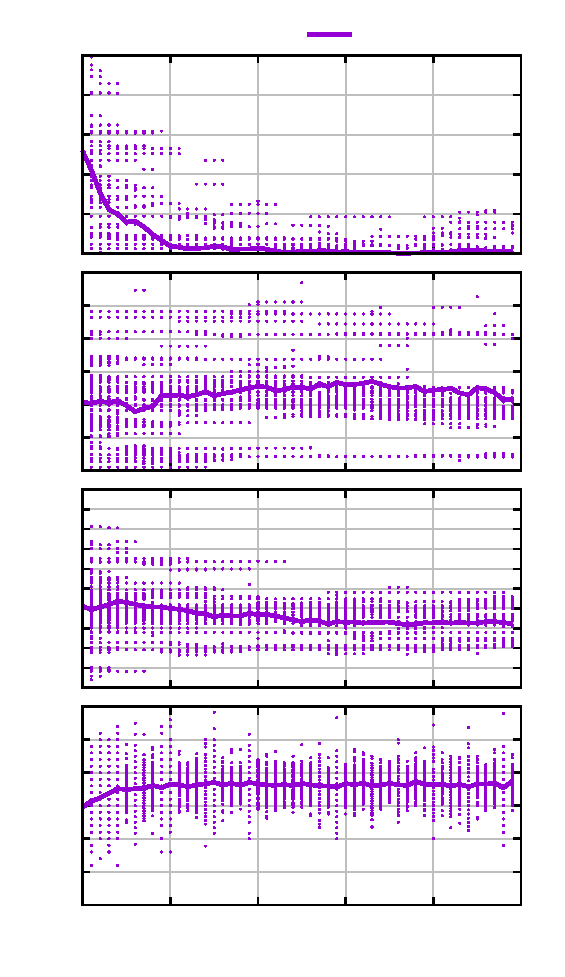
\includegraphics{pictures/top_optimization}}%
    \gplfronttext
  \end{picture}%
\endgroup
}
    \caption{
        Genetic optimization of genotypes with an fraction $q$ of Erd�s-Renyi
        topology and $1-q$ of ring topology for the challenge $C\ix{high}$.
        This figure is to be understood like FIG. \ref{fig:freq_optimization}.
    }
    \label{fig:top_optimization}
\end{figure}


\section{Discussion}
%- Remarks
    %* Influence of initial conditions
        %-> Degenerated initial population poses major problems (does not
        %find same / takes very long to find same parameters as when started
        %with diversity).
        %-> With broad diversity: often fast convergence -> Gen. Optimizer
        %good as optimizing filter, but has hard times to explore new
        %parameter regions if no right genotypes are present (especially isolated
        %maxima of $F_C$). Solution: Could introduce migrants, that supply
        %the gene-pool with underrepresented genotypes.
    %* According to experience: maybe not ideal for finding single set of
      %parameters but rather for successful parameter-ranges (branches?)


%- Problems
    %* Only few and uncomprehensive number of test / experiments conducted due to the
      %computational cost.
    %* Influence of statistics: Learning success depends stronger on choice
      %of challenges than parameters (partially) -> must be very careful how to
      %interpret the results / should have used fixed array of challenges instead
      %of random sampling

%Our investigation showed that the frequency of sinusoidal tasks strongly
%determines whether FORCE learning is able to learn it or not. Still, a good
%choice of network parameters, conveying structural information, is able to
%improve the success rate for certain frequency ranges. 
%Under certain conditions, some parameters (like $\ERprob$ for low
%frequencies or $\feedback$ for high frequencies) can vary in a relatively
%large interval without influencing the success critically.

While we only presented results concerning simple sinusoidals of varying
frequencies in this article, the code developed during our project provides
a framework which can be used to perform a variety of similar and extended
investigations; for example the inclusion of feed forward topologies and
arbitrary (higher dimensional) tasks with optional external input pathways
(e.g.\ as a timer signal to make the network synchronize better).

One peculiarity to be recognized throughout our project work is that the
optimization algorithm does not excel at providing strictly converging,
single most optimal parameter values, but that we are rather given more or
less broad ``survival ranges'' for each parameter as result. And though the
final genotypes vary quite a bit in their fitness, we did not observe
strong correlations between the different parameters in these ranges when
doing sporadic tests.

Indeed, looking at all of our simulations in their entirety, the genotype
parameters show less influence on the learning results than we initially
expected, and during our inquiry it often seamed that the statistics of the
challenges might overshadow the effect of the parameters -- at least when
looking at more complex tasks than monofrequent waves. A wise improvement
would therefore be to make the challenges more deterministic, e.g.\ to use
the same tasks for all genotypes in each generation instead of drawing them
independently from some (wide range) distribution.

Another issue to be mentioned with the current implementation is the large
amount of empirical (``magic") numbers, i.e.\ hyper-parameters of the
optimization used in the code. Examples hereof are the strength of the
mutation process or the mechanics of the selection process (actual number
of survivors, survival chances for weaker genotypes, etc.).  Their values
were determined by an informal search of testing a few optimizations but
were not investigated thoroughly. This should, however, mostly affect the
performance of the optimization algorithm and not the results themselves. 

%One problem with the approach presented here is that, in order to use the
%results of the genetic algorithm, we determined a single set of parameters
%by taking the mean of the values of the most successful generators.
%Thereby, any information about an interdependence between the parameters
%is lost. We checked that there are no strong correlations between any pair
%of parameters by doing 3D plots that showed the two parameters for each
%generator in development with the generations and could not detect any
%obvious correlation, but have not investigated this problem thoroughly. 

Nevertheless we were able to produce successful optimization results
and could indeed show that adaption to high frequencies can not only be
accomplished by an implausible effect, namely the 
high feedback values, but also by changing the topological structure of the
network. In this regard it would certainly be interesting to further
inquire how genotypes that allow for a more fine grained control over the
topology behave under the optimization.

%This would certainly make the selection process more robust as it removes
%the dependence of the task distributions.
%In general, the genotypes parameters showed less influence than we expected.
%, whereas others are
%restricted to more concise regions (???).
%Some parameters
%($\ERprob$, $\feedback$) can vary in a relatively large interval without
%influencing the success very much, whereas others are confined to
%a relatively small interval ($\gain$).

%To that end, it would be wise to improve that selection
%algorithm by using the same tasks
%for all generators in each generation, instead of evaluating them all independently. This would make the 
%selection process more robust because it removes the dependence on the task distribution. 

%One problem with the approach presented here is that, in order to use the results of the genetic algorithm, 
%we determined a single set of parameters by taking the mean of the values of the most successful generators.
%Thereby, any information about an interdependence between the parameters is lost. We checked that there are no strong
%correlations between any pair of parameters by doing 3D plots that showed the two parameters for each generator 
%in development with the generations and could not detect any obvious correlation, but have not investigated 
%this problem thoroughly. 


\bibliography{sources}

\end{document}
